% =============================================================
% บทที่ 2 - ทฤษฎีและงานวิจัยที่เกี่ยวข้อง
% =============================================================

% -----------------------------------------------------------
\section{ทฤษฎีที่เกี่ยวข้อง}
% -----------------------------------------------------------

\subsection{กระบวนการวิทยาการข้อมูลและการจัดทำท่อส่งข้อมูล (Data Science \& Pipeline Process)}

กระบวนการวิทยาการข้อมูลเป็นกรอบการทำงานเชิงระบบที่นำข้อมูลขนาดใหญ่มาประมวลผลและวิเคราะห์ เพื่อค้นหารูปแบบหรือสร้างคุณประโยชน์ ในโครงงานนี้ได้ประยุกต์ใช้กระบวนการ 5 ขั้นตอน ร่วมกับการออกแบบท่อส่งข้อมูลแบบโมดูลาร์ (Modular Data Pipeline) ได้แก่

\begin{enumerate}[label=\arabic*)]
    \item \textbf{การกำหนดวัตถุประสงค์และคำถามวิจัย (Question Refinement):} กำหนดโจทย์ในการทำนายผลการแข่งขันฟุตบอลพรีเมียร์ลีกอังกฤษออกเป็น 3 รูปแบบ ได้แก่ ทีมเจ้าบ้านชนะ (Home Win: H), เสมอ (Draw: D) และทีมเยือนชนะ (Away Win: A)
    \item \textbf{การเก็บรวบรวมข้อมูลและการดึงข้อมูลแบบหลายแหล่ง (Data Collection \& Multi-Source Scraping):} การสร้างระบบดึงข้อมูลอัตโนมัติเพื่อสแครปข้อมูลสถิติการแข่งขัน อัตราต่อรอง รายชื่อผู้เล่น 11 ตัวจริง มูลค่าการตลาด และสถิติลายบุคคลจากหลายแหล่งสาธารณะ ได้แก่ FBref, Understat, Transfermarkt และ Kaggle \cite{kaggle2024, fbref2024, transfermarkt2024, understat2024}
    \item \textbf{การสำรวจ ตรวจสอบ และสร้างตัวแปร (Data Validation \& Feature Engineering):} การตรวจสอบคุณภาพข้อมูลผ่านสัญญาข้อมูล (Data Contracts) การจัดการค่าที่ขาดหาย การทำกระบวนการจัดสเปกเอนทิตี (Entity Resolution) เพื่อจับคู่ชื่อสโมสร และการสร้างตัวแปรใหม่ เช่น คะแนน Elo Difference, ค่า xG ย้อนหลัง (Rolling xG) และดัชนีความเหนื่อยล้าสะสมของนักเตะ (Fatigue Metric)
    \item \textbf{การสร้างและประเมินแบบจำลอง (Model Building \& Evaluation):} การฝึกฝนโมเดลการเรียนรู้ของเครื่อง และประเมินประสิทธิภาพด้วยตัวชี้วัดต่าง ๆ เช่น Accuracy, Log Loss และ F1-Score \cite{scikit-learn}
    \item \textbf{การสรุปและวิเคราะห์ผลลัพธ์ (Communication \& Feature Analysis):} การสรุปผลการวิเคราะห์ เปรียบเทียบประสิทธิภาพกับราคาอัตราต่อรองของตลาด และนำเสนอระดับความสำคัญของตัวแปรทำนาย (Feature Importance)
\end{enumerate}

\subsection{ระบบวัดระดับความแข็งแกร่ง (Elo Rating System)}

ระบบคะแนน Elo เป็นวิธีทางสถิติที่ใช้คำนวณระดับทักษะความแข็งแกร่งของทีมแข่งขัน คะแนนจะถูกปรับเปลี่ยนตามผลการแข่งขันจริงและระดับความแข็งแกร่งของคู่แข่ง โดยทีมที่ชนะทีมที่มีคะแนนสูงกว่าจะได้คะแนนเพิ่มขึ้นมากกว่าการชนะทีมที่อ่อนกว่า \cite{hvattum2010using} ในโครงงานนี้ ได้มีการคำนวณค่า Elo Rating ของแต่ละสโมสรอย่างต่อเนื่องตามลำดับเวลา (Time-series) ดังแสดงในรูปที่ \ref{fig:elo_concept} และนำผลต่างคะแนน Elo (Elo Difference) ระหว่างทีมเจ้าบ้านและทีมเยือนมาใช้เป็นฟีเจอร์สำคัญในการสะท้อนความได้เปรียบเชิงศักยภาพของทีม

\begin{figure}[H]
    \centering
    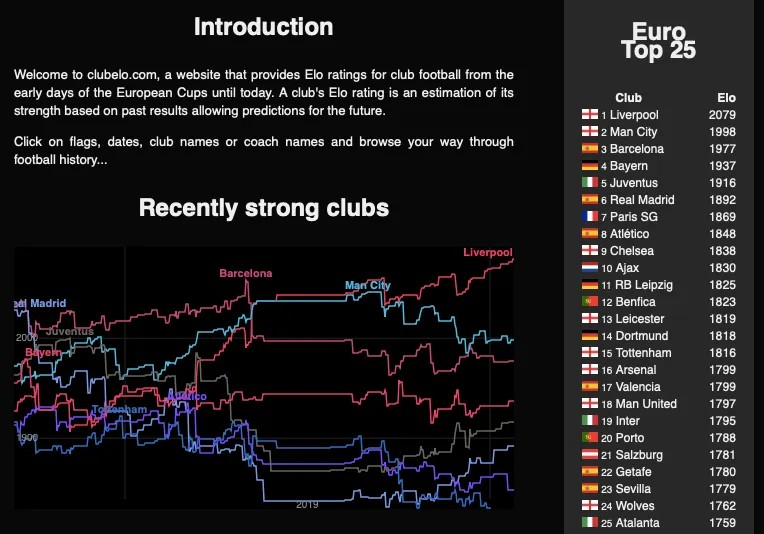
\includegraphics[width=0.8\textwidth]{images/elo_concept.jpg}
    \caption{ตัวอย่างแผนภาพแสดงการปรับปรุงคะแนน Elo Rating ของสโมสรฟุตบอลตามผลการแข่งขันย้อนหลัง (ที่มา: ClubElo)}
    \label{fig:elo_concept}
\end{figure}

\subsection{ค่าความคาดหวังในการทำประตู (Expected Goals: xG)}

ค่า xG เป็นตัวชี้วัดเชิงสถิติขั้นสูงที่ใช้ประเมินคุณภาพของโอกาสในการยิงประตู โดยคำนวณความน่าจะเป็นที่ลูกยิงแต่ละครั้งจะกลายเป็นประตู (มีค่าระหว่าง 0 ถึง 1) ขึ้นอยู่กับตำแหน่งการยิง มุมในการยิง ประเภทการส่งบอล และบริบทของเกม ดังแสดงตัวอย่างในรูปที่ \ref{fig:xg_concept} ค่า xG ช่วยให้มองเห็นประสิทธิภาพเกมรุก (xG) และเกมรับ (Expected Goals Against: xGA) ที่แท้จริงของทีม ซึ่งสะท้อนฟอร์มการเล่นได้ดีกว่าผลสกอร์แพ้-ชนะแบบดั้งเดิม \cite{understat2024}

\begin{figure}[H]
    \centering
    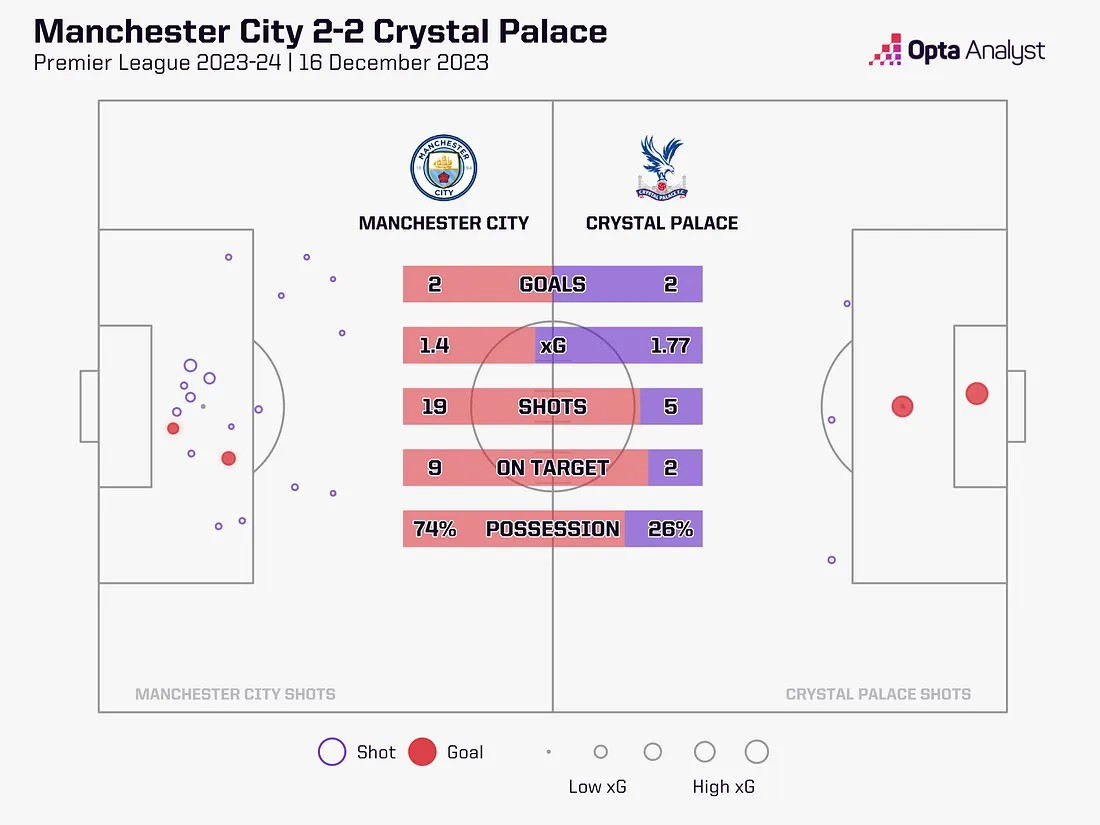
\includegraphics[width=0.8\textwidth]{images/xg_shot_map.jpg}
    \caption{ตัวอย่างการประเมินค่าความคาดหวังในการทำประตู (Expected Goals: xG) จากตำแหน่งการยิง (ที่มา: Opta Analyst)}
    \label{fig:xg_concept}
\end{figure}

\subsection{ดัชนีความเหนื่อยล้าและความตึงของตารางแข่ง (Fatigue Metric \& Schedule Congestion)}

ระยะเวลาพักผ่อนระหว่างแมตช์การแข่งขันส่งผลต่อสภาพร่างกายและประสิทธิภาพการเล่นของนักเตะอย่างมีนัยสำคัญ ในโครงงานนี้ได้ประยุกต์ใช้ทฤษฎีการวิเคราะห์ความเหนื่อยล้าสะสม โดยคำนวณจากจำนวนวันพัก (Days Rest) ระหว่างการแข่งขันนัดปัจจุบันกับนัดก่อนหน้า ควบคู่กับดัชนีความหนาแน่นของโปรแกรมการแข่งขันและระดับความยากของโปรแกรมแข่งขัน (ดังแสดงในรูปที่ \ref{fig:fatigue_concept}) เพื่อให้แบบจำลองสามารถรับรู้ถึงปัจจัยความเหนื่อยล้าของทีมที่ต้องลงเล่นในตารางการแข่งขันที่แน่นหนา

\begin{figure}[H]
    \centering
    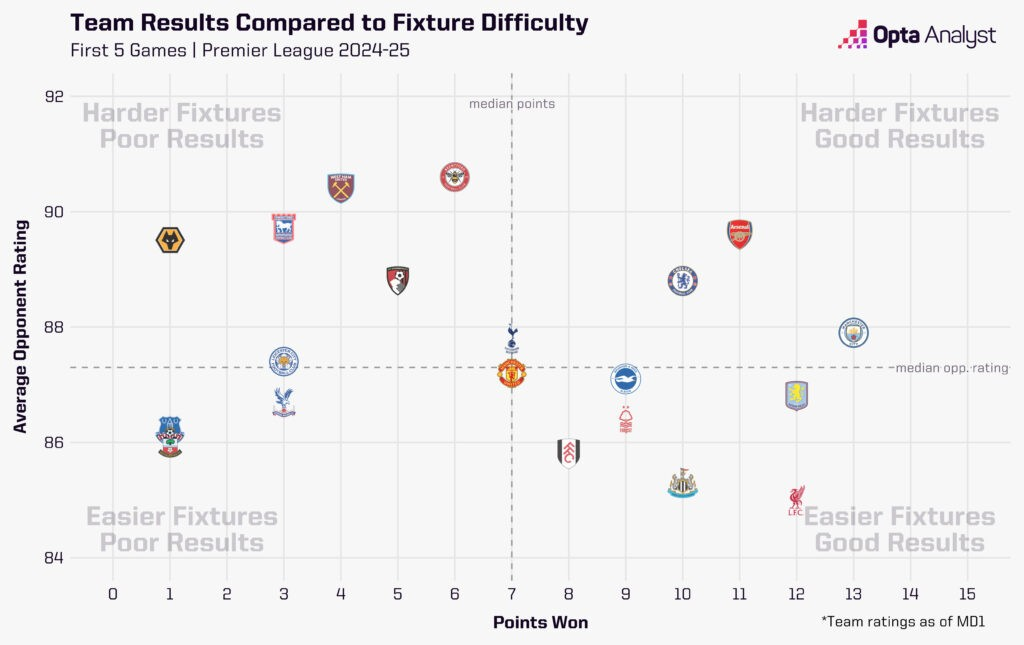
\includegraphics[width=0.8\textwidth]{images/fatigue_concept.jpg}
    \caption{ตัวอย่างการวิเคราะห์ความตึงเครียดของโปรแกรมแข่งขันและระดับความแข็งแกร่งของทีมคู่แข่ง}
    \label{fig:fatigue_concept}
\end{figure}

\subsection{อัตราต่อรองของเจ้ามือรับพนัน (Betting Market Odds)}

อัตราต่อรองในตลาดเดิมพันนอกจากจะใช้ในเชิงการพนันแล้ว ในทางวิทยาการข้อมูลยังถือเป็นตัวชี้วัดความน่าจะเป็น (Implied Probability) ที่ผ่านการประมวลผลข้อมูลเชิงลึกและปัจจัยแวดล้อมโดยผู้เชี่ยวชาญ \cite{dixon1997modelling} ในโครงงานนี้ ราคาอัตราต่อรองสำหรับผลการแข่งขัน 3 รูปแบบ จะถูกแปลงให้อยู่ในรูปของค่าความน่าจะเป็น เพื่อใช้เป็นตัวแปรนำเข้าควบคู่กับสถิติการเล่น และใช้เป็นเกณฑ์อ้างอิงมาตรฐาน (Benchmark) ในการเปรียบเทียบประสิทธิภาพกับแบบจำลองที่พัฒนาขึ้น \cite{hubacek2021forty}

\subsection{การจับคู่และแปลงชื่อเอนทิตีให้เป็นมาตรฐาน (Entity Resolution)}

เนื่องจากข้อมูลถูกรวบรวมมาจากหลายแหล่งข้อมูลภายนอก ทำให้ชื่อสโมสรฟุตบอลเดียวกันอาจถูกบันทึกด้วยข้อความที่แตกต่างกัน (เช่น \texttt{"Man Utd"}, \texttt{"Manchester Utd"} และ \texttt{"Manchester United"}) กระบวนการ Entity Resolution จึงถูกนำมาใช้เพื่อปรับแปลงชื่อทีมจากทุกแหล่งข้อมูลให้อยู่ในรูปแบบมาตรฐาน (Canonical Team Names) ผ่าน Dictionary Mapping และตารางดรรชนี เพื่อให้การเชื่อมโยงข้อมูล (Data Joining) มีความถูกต้องสมบูรณ์ 100\%

\subsection{การจำแนกประเภทด้วยการเรียนรู้ของเครื่อง (Machine Learning Classification)}

การทำนายผลการแข่งขันฟุตบอลถูกกำหนดให้เป็นโจทย์การจำแนกประเภทแบบหลายกลุ่ม (Multiclass Classification) 3 กลุ่ม ได้แก่ ทีมเจ้าบ้านชนะ (Home Win: H), เสมอ (Draw: D) และทีมเยือนชนะ (Away Win: A) โดยเลือกใช้แบบจำลองผ่านไลบรารี Scikit-learn \cite{scikit-learn} ดังนี้

\paragraph{1) Logistic Regression}
เป็นแบบจำลองเชิงเส้นทางสถิติที่ใช้วิเคราะห์ความน่าจะเป็น เหมาะสำหรับใช้เป็นแบบจำลองพื้นฐาน (Baseline Model) เนื่องจากคำนวณได้เร็ว ไม่ซับซ้อน และตีความผลลัพธ์ผ่านค่าสัมประสิทธิ์ของตัวแปรได้ง่าย

\paragraph{2) Decision Tree}
เป็นแบบจำลองโครงสร้างต้นไม้ที่ตัดสินใจแบ่งข้อมูลตามเงื่อนไขของตัวแปรตามเกณฑ์ เช่น Gini Impurity หรือ Information Gain มีจุดเด่นคือเข้าใจเงื่อนไขการทำงานได้ง่าย แต่เสี่ยงต่อปัญหาการเรียนรู้ดีเกินไป (Overfitting)

\paragraph{3) Random Forest}
เป็นเทคนิค Ensemble Learning ที่สร้าง Decision Tree จำนวนหลายต้นและใช้วิธีรวมผลการตัดสินใจ (Majority Voting) เพื่อสรุปผลการตัดสินใจ ช่วยลดปัญหา Overfitting เพิ่มความแม่นยำ และสามารถวัดระดับความสำคัญของตัวแปร (Feature Importance) ได้ดี \cite{berrar2019incorporating}

% -----------------------------------------------------------
\section{งานวิจัยที่เกี่ยวข้อง}
% -----------------------------------------------------------

ในส่วนนี้เป็นการทบทวนวรรณกรรมและงานวิจัยที่นำเทคนิควิทยาการข้อมูลและการเรียนรู้ของเครื่องมาใช้ในการทำนายผลกีฬา เพื่อหาแนวทางและช่องว่างในการพัฒนาโครงงาน

\subsection{การทำนายผลฟุตบอลด้วยแบบจำลองเชิงสถิติและอัตราต่อรอง}

งานวิจัยยุคแรกมักใช้สถิติการแข่งขันย้อนหลัง เช่น จำนวนประตูที่ทำได้ ฟอร์มเหย้า-เยือน ผ่านโมเดลเชิงสถิติตระกูล Poisson \cite{dixon1997modelling} หรือระบบจัดอันดับ Rating \cite{hvattum2010using, constantinou2013determining} ซึ่งจากการประเมินและทบทวนวรรณกรรมย้อนหลัง 40 ปีโดย Hubáček และคณะ \cite{hubacek2021forty} ที่ทดสอบกับชุดข้อมูลกว่า 2.1 แสนนัด พบว่าแบบจำลองที่ใช้เพียงผลสกอร์ย้อนหลังมีขีดจำกัดความแม่นยำอยู่เพียงร้อยละ 47.8--48.6 เท่านั้น ในขณะที่ราคาอัตราต่อรองจากตลาดเดิมพันกลับให้ความแม่นยำสูงกว่า (ประมาณร้อยละ 53--55) เนื่องจากสะท้อนข้อมูลเชิงลึกในตลาดได้อย่างรวดเร็ว อย่างไรก็ตาม การใช้เพียงอัตราต่อรองอย่างเดียวจะไม่สามารถอธิบายปัจจัยภายในหรือบริบทการเล่นของทีมได้ครบถ้วน

% \begin{figure}[H]
%     \centering
%     \includegraphics[width=0.8\textwidth]{images/hubacek_season_error.png}
%     \caption{การเปรียบเทียบค่าความคลาดเคลื่อน (Cross-entropy) ของแบบจำลองทำนายผลฟุตบอลประเภทต่างๆ ตามสัดส่วนของฤดูกาล (ที่มา: Hubá\v{c}ek et al., 2021)}
%     \label{fig:hubacek_season_error}
% \end{figure}

\subsection{การใช้ Machine Learning ร่วมกับการวิเคราะห์ตัวแปรสถิติเชิงลึกและรายชื่อผู้เล่น}

งานวิจัยหลายฉบับทดลองใช้อัลกอริทึม Logistic Regression, Decision Tree และ Random Forest ในการทำนายผลฟุตบอล โดยใช้สถิติการครองบอล การยิงประตู และฟอร์มย้อนหลัง ซึ่งพบว่า Random Forest มักให้ผลลัพธ์ที่ดีกว่าโมเดลเชิงเส้น อย่างไรก็ตาม งานวิจัยส่วนใหญ่มักมองข้ามปัจจัยด้านผู้เล่นและมูลค่าทีม เช่น ข้อมูลไลน์อัปจริง ค่าความเหนื่อยล้า และมูลค่าการตลาดสโมสร ซึ่ง Berrar และคณะ \cite{berrar2019incorporating} ได้ชี้ให้เห็นว่าการดึงข้อมูลเฉพาะทางและบริบทแวดล้อม (Domain Knowledge) เช่น สถิติ xG และไลน์อัปตัวจริง เข้ามาประกอบ จะช่วยให้โมเดล Machine Learning ทำนายผลได้แม่นยำยิ่งขึ้น

\subsection{สรุปผลการเปรียบเทียบงานวิจัยที่เกี่ยวข้อง}

จากการทบทวนวรรณกรรม สามารถสรุปเปรียบเทียบองค์ประกอบระหว่างแนวทางงานวิจัยทั่วไปกับโครงงานนี้ได้ดังตารางที่ \ref{tab:compare_research}

\begin{table}[htbp]
\centering
\caption{การเปรียบเทียบองค์ประกอบของงานวิจัยที่เกี่ยวข้องกับโครงงานนี้}
\label{tab:compare_research}
\resizebox{\textwidth}{!}{%
\begin{tabular}{|l|c|c|c|c|c|}
\hline
\textbf{การศึกษา / โครงงาน} & \textbf{สถิติผลสกอร์} & \textbf{อัตราต่อรอง} & \textbf{Elo / xG} & \textbf{มูลค่าทีม / ไลน์อัป} & \textbf{ดัชนีความเหนื่อยล้า} \\
\hline
งานวิจัยที่เน้นสถิติการแข่งขัน \cite{dixon1997modelling, hubacek2021forty} & \checkmark & -- & -- & -- & -- \\ \hline
งานวิจัยที่เน้นอัตราต่อรองตลาด \cite{constantinou2013determining} & \checkmark & \checkmark & -- & -- & -- \\ \hline
งานวิจัยใช้แบบจำลอง ML เบื้องต้น \cite{hvattum2010using, berrar2019incorporating} & \checkmark & -- & \checkmark & -- & -- \\ \hline
\textbf{โครงงานนี้} & \checkmark & \checkmark & \checkmark & \checkmark & \checkmark \\
\hline
\end{tabular}%
}
\end{table}

จากตารางที่ \ref{tab:compare_research} จะเห็นว่าโครงงานนี้ได้บูรณาการทั้งสถิติการแข่งขัน ราคาอัตราต่อรอง ตัวชี้วัดขั้นสูง (Elo, xG) มูลค่าการตลาดสโมสร รายชื่อไลน์อัป และดัชนีความเหนื่อยล้าเข้าด้วยกัน เพื่อวิเคราะห์ปัจจัยที่มีผลต่อการแข่งขันอย่างครอบคลุมยิ่งขึ้น

% -----------------------------------------------------------
\section{เครื่องมือและเทคโนโลยีที่ใช้}
% -----------------------------------------------------------

\subsection{ภาษา Python และไลบรารีสำหรับการประมวลผลข้อมูล}

ภาษา Python เป็นภาษาหลักที่ใช้ในการดำเนินโครงงาน เนื่องจากมีระบบนิเวศของไลบรารีที่สนับสนุนงานด้าน Data Science และ Data Engineering อย่างครบถ้วน ได้แก่

\begin{enumerate}[label=\arabic*)]
    \item \textbf{Polars และ Pandas:} ใช้สำหรับการจัดการ จัดเตรียม ดึงข้อมูล ทำความสะอาด และประมวลผลตารางข้อมูลประสิทธิภาพสูง (High-performance DataFrames) \cite{pandas2010}
    \item \textbf{Pandera และ Pydantic:} ใช้สำหรับการตรวจสอบความถูกต้องของโครงสร้างข้อมูล (Data Schema Validation \& Data Contracts) ในขั้นตอนรับข้อมูลดิบและล้างข้อมูล
    \item \textbf{Scikit-learn:} ใช้พัฒนาแบบจำลองการเรียนรู้ของเครื่อง (Logistic Regression, Decision Tree, Random Forest) การแบ่งชุดข้อมูลแบบลำดับเวลา (Temporal Split) และการประเมินวัดผล \cite{scikit-learn}
    \item \textbf{Matplotlib และ Seaborn:} ใช้ในการทำ Data Visualization เพื่อสำรวจข้อมูลและแสดงผลกราฟความสำคัญของตัวแปร (Feature Importance)
\end{enumerate}

\subsection{สภาพแวดล้อมและการประกันคุณภาพซอฟต์แวร์ (Development Environment \& Quality Control)}

\begin{enumerate}[label=\arabic*)]
    \item \textbf{ระบบบริหารจัดการสภาพแวดล้อมเสมือน (\texttt{uv}):} เครื่องมือบริหารจัดการ Virtual Environment และไลบรารีความเร็วสูง ช่วยควบคุมรุ่นของไลบรารีให้สอดคล้องกันตลอดกระบวนการพัฒนา
    \item \textbf{ระบบทดสอบซอฟต์แวร์และตรวจสอบโค้ดอัตโนมัติ (Pytest \& Ruff):} ใช้สำหรับการเขียนและรันชุดทดสอบความถูกต้องอัตโนมัติ (Unit Testing) ในท่อส่งข้อมูล และการตรวจสอบมาตรฐานรูปแบบโค้ด
    \item \textbf{แหล่งชุดข้อมูลสาธารณะ (FBref, Understat, Transfermarkt, Kaggle):} เป็นแหล่งจัดเก็บข้อมูลผลการแข่งขัน อัตราต่อรอง สถิติ xG รายชื่อไลน์อัป 11 ตัวจริง และมูลค่าการตลาดของนักเตะ \cite{kaggle2024, fbref2024, transfermarkt2024, understat2024}
\end{enumerate}